\documentclass[20pt]{beamer}

\input{poster_preamble}
\usepackage[size=a0,orientation=portrait, scale=1.4]{beamerposter}

%\defbeamertemplate{headline}{
%%\beamercolorbox[wd=\paperwidth]{chcolor}
%\begin{columns}
%
%\begin{column}{width=.15\linewidth}
%Boy
%\end{column}
%\begin{column}{width=.85\linewidth}
%Hello
%\end{column}
%\end{columns}
%
%}






\begin{document}


\begin{frame}%[t]
\frametitle{\Huge
\begin{center}
\vspace{100pt}

Quantum theory of radiation for nonstationary systems \par\vspace{50pt}
\Large
Frederic Ongonwou and Toru Morishita \par\vspace{30pt}
Department of Engineering Science, The University of Electro-Communications
\end{center}
}

\framesubtitle{
\begin{center}
\small 
High harmonic generation (HHG) and photoelectron momentum distribution (PEMD) 
are some of the most 
important processes driving the study of matter-radiation interaction
and will lead to important advances in fundamental science and engineering.
Through HHG, for example, it is possible to produce coherent radiations 
outperforming the external fields in regards to frequency and pulse duration.
The current theory, valid for stationary systems, falls short at
the description of nonstationary systems, since it ignores radiations
induced by the external force. 
Following Yangaliev \textit{et al.}[1], we aim at 
extending the quantum theory of radiation for real nonstationary systems,
i.e in 3 dimensions and for realistic potentials.
\end{center}
}

% ----- First column

\begin{textblock*}{\textwidth}(100pt,800pt)
{\huge\textbf {1. Background}} \\\vspace{30pt}
%Theory and illustrations to put here

\end{textblock*}

\begin{textblock*}{700pt}(100pt,900pt)
%\centering
%\rotatebox{90}{
  \small \textbf{Basic strong field phenomena}
 \begin{minipage}{0.6\linewidth}
 \begin{figure}[tp]
 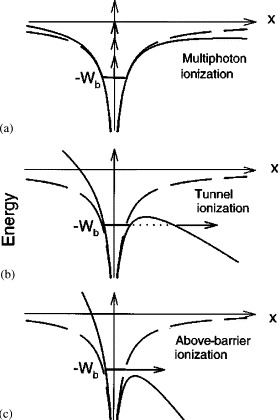
\includegraphics[scale=1., trim={0 0 0 0},clip]{images/phenomena.png} \\
%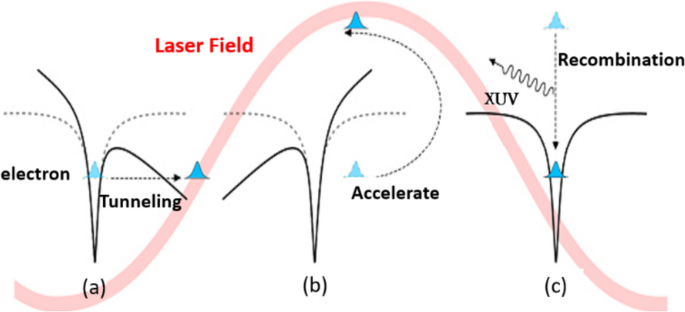
\includegraphics[scale=.50, trim={0 0 0 0},clip]{images/hhg_process.png}

%%\caption{Eigenvalues.}
%\label{fig:pemd_0114}
 \end{figure}

\end{minipage}
\end{textblock*}


\begin{textblock*}{500pt}(500pt,1000pt)
%\centering
%\rotatebox{90}{
 \begin{minipage}{0.5\linewidth}
%  \scriptsize Basic strong field phenomena
 \begin{figure}[tp]
%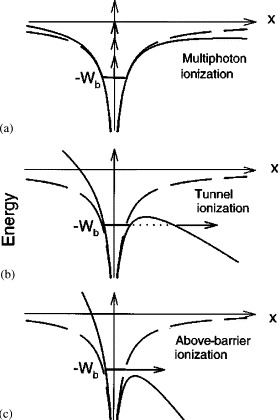
\includegraphics[scale=1., trim={0 0 0 0},clip]{images/phenomena.png} \\
 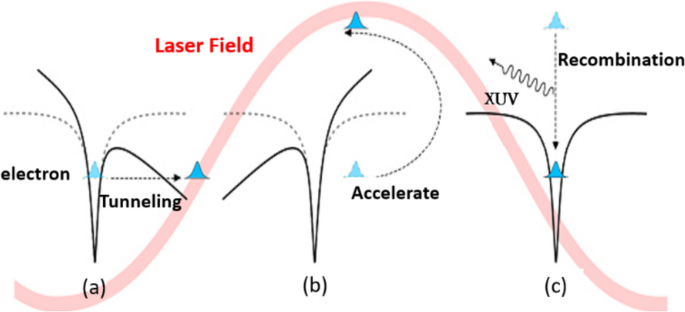
\includegraphics[scale=.50, trim={0 0 0 0},clip]{images/hhg_process.png} \\
\vspace{10pt}
 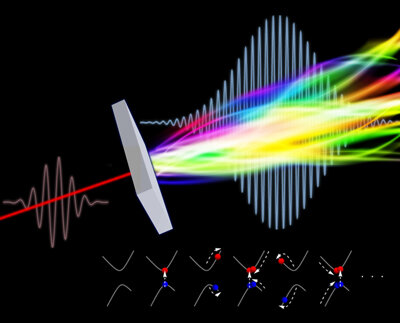
\includegraphics[scale=1.1, trim={0 80 0 0},clip]{images/modeling-high-harmonic.jpg}
%\caption{Eigenvalues.}
%\label{fig:pemd_0114}
 \end{figure}

\end{minipage}
\end{textblock*}




\begin{textblock*}{0.41\textwidth}(100pt,1400pt)
{\huge\textbf {2. Goal}} \\\vspace{30pt} 
{\small \textbf{Full quantum treatment of the HHG theory} \\
Schr\"odinger equation
\begin{align}
 i\frac{\partial \left| \Psi(t)\right\rangle}{\partial t}
 =   \Bigg[ \hat{H}_{\rm a}
  \ + \hat{H}_{\rm f} \Bigg.
 & \Bigg. + \alpha \boldsymbol{\hat{\rm A}\hat{\rm p}}
 + \hat{V}_{\rm ext}(t)
\Bigg]
\left|\Psi(t)\right\rangle, \nonumber\\
 \begin{split}
 \left|\Psi(t)\right\rangle = \sum_n  & A_n(t) 
 e^{-iE_n t}\left| \psi_n^-,0\right\rangle \\
 & + \alpha \sum_{n\nu} B_{n\nu}(t) 
 e^{-i\left(E_n + \omega\right) t}\left| \psi_n^-,\nu\right\rangle. \nonumber
\end{split}
\end{align}
}
\vspace{20pt}

{\footnotesize
\begin{align}
\left| \psi_n^-,0\right\rangle & =
\left| \psi_n^-\right\rangle\left|0\right\rangle 
  + i\alpha\sum_\nu \hat{R}_\nu 
      \left| \psi_n^- \right\rangle \left| \nu \right\rangle 
               + O(\alpha^2), \nonumber\\
\left| \psi_n^-,\nu\right\rangle & =
\left| \psi_n^-\right\rangle\left|\nu\right\rangle 
  - i\alpha \hat{R}_\nu^\dagger 
  \left| \psi_n^-\right\rangle \left|\nu\right\rangle
     + \alpha \times \mbox{(two-photons states)} + O(\alpha^2). \nonumber
\end{align}
}

{\normalsize
{\small PEMD and HHG in a full quantum treatment } \\
\begin{equation}
%P_n = \left| \left\langle \psi_n^-,0 |
%     \Psi(t\leqslant T)\right\rangle\right|^2,
% \hspace{10pt}
%Q_\nu = \sum_n \left| \left\langle \psi_n^-, \nu | 
%    \Psi(t\leqslant T)\right\rangle\right|^2.
%P_n = \left| A_n \right|^2,
P_n = \left| \left\langle \psi_n^-,0 
  | \Psi(t\geqslant T)\right\rangle\right|^2,
 \hspace{30pt}
%Q_\nu = \sum_n \left\langle \Psi(t) | 
%  \bar{d}_\nu^\dagger \bar{d}_\nu | \Psi(t)\right\rangle|_{t\geqslant T}.
Q_\nu = \sum_n \left| \left\langle \psi_n^-,\nu 
  | \Psi(t\geqslant T)\right\rangle\right|^2.
 \nonumber
\end{equation}}
{
\small \noindent These observables are usually evaluated 
at the order 0 of the perturbation theory $(\alpha \longrightarrow 0)$,
between some more approximations}
\end{textblock*}


\begin{textblock*}{400pt}(50pt,1650pt)
\scriptsize
\begin{align}
&\hat{H}_{\rm a} = \frac{\hat{\boldsymbol{\rm p}}^2}{2} + \hat{V}_{\rm a} \nonumber\\
&\hat{H}_{\rm a} \left|\psi_n^{\pm}\right\rangle = E_n \left|\psi_n^{\pm}\right\rangle\nonumber \\
& \hat{H}_{\rm f} =  \sum_{\nu} \omega \hat{a}_\nu^\dagger \hat{a}_\nu,
\hspace{30pt} \hat{H}_{\rm f}\left|\nu\right\rangle = 
\omega \left|\nu\right\rangle \nonumber\\
& \hat{R}_\nu = \int e^{i\hat{H}_{\rm a}t}\boldsymbol{\hat{\rm A}}_\nu
\boldsymbol{\hat{\rm p}} e^{-i\hat{H}_{\rm a}t}
e^{i\omega t - \epsilon t} dt
\nonumber
\end{align}
\end{textblock*}


\begin{textblock*}{0.42\textwidth}(100pt,2300pt)
{\huge\textbf {3. Illustration}} \\\vspace{30pt}
{\small The classical ansatz (semi-classical treatment)}
\begin{align}
 & i\frac{\partial \psi(x,t)}{\partial t}
 =  \left[ -\frac{1}{2}\frac{d}{dx^2} -\varkappa\delta(x)  %+ \hat{V}_{\rm a}
 + F(t)x\right]\psi(x,t),  \hspace{20pt} \nonumber\\
& i\frac{\partial \phi_\omega(x,t)}{\partial t}
 =  \left[ -\frac{1}{2}\frac{d}{dx^2} -\varkappa\delta(x) +  F(t)x\right]\phi_\omega(x,t)
  + e^{i\omega t}\hat{p}\,\psi(x,t), \hspace{40pt}  \\
   & \mbox{ \footnotesize $\phi_\omega (x,0) = \frac{-i\varkappa^{3/2}}{\omega}
{\rm sgn}(x)\left(e^{-\varkappa|x|} - e^{-\varkappa(\omega)|x|}\right),
\hspace{20pt}  \psi(x,0) = \varkappa^{1/2}e^{-\varkappa|x|}$, 
\hspace{40pt}\footnotesize $E_0 = -\varkappa^2/2$.}\nonumber
\end{align}

{\footnotesize
\begin{align}
 & a_0 = e^{iE_k t} \int \psi(x,0)\psi(x,T)dx, \hspace{150pt}
 a_k = e^{iE_k t} \int \psi_k^{(-)*}(x)\psi(x,T)dx, \nonumber \\
 & b_{0\omega} = b_{0\omega}(T) 
+ \int \frac{e^{i(E_0+\omega-E_{k^\prime})T}
p_{0k^\prime}a_{k^\prime}}{E_0 + \omega -E_{k^\prime} + i0}
\frac{dk^\prime}{2\pi},\nonumber \\
& b_{k\omega} = b_{0\omega}(T) +  \frac{e^{i(E_0+\omega-E_0)T}p_{k0}a_0}
{E_k + \omega +-E_0}
+ \int \frac{e^{i(E_k+\omega-E_{k^\prime})T}
p_{kk^\prime}a_{k^\prime}}{E_k + \omega -E_{k^\prime} + i0}
\frac{dk^\prime}{2\pi}r. \nonumber
\end{align}
}
\vspace{10pt}
Convergence assessment observables
\begin{equation}
\rho(x,t) = \left| \psi(x,t) \right|^2, \hspace{150pt}
P_0 = \left| a_0 \right|^2, \hspace{100pt}
P_0 + P_{\rm ion} = 1. \nonumber
\end{equation}

Alternative PEMD and HHG expressions in the classical ansatz[1]
\begin{equation}
P(k) = \left| a_k \right|^2, \hspace{100pt}
Q_\nu^{(c)} = \alpha^2\omega^2
   \left| \boldsymbol{\rm A}_\nu \boldsymbol{\rm d}(\omega)\right|^2 \nonumber
\end{equation}

%\scriptsize
%\begin{equation}
%\hspace{200pt}
%d(t) = - \left\langle \psi (t)| \hat{x} |\psi(t) \right\rangle, \hspace{30pt}
%d(\omega) = \int e^{i\omega t} d(t) dt
% \nonumber
%\end{equation}


\end{textblock*}

\begin{textblock*}{\textwidth}(70pt,3250pt)
{\normalsize\textbf {References}} \\\vspace{20pt}
\end{textblock*}

\begin{textblock*}{\textwidth}(300pt,3250pt)
\scriptsize
 $[1]$ D. N. Yangaliev, V. P. Krainov and O. I. Tolstikhin, 
Phys. Rev. A 101, 013410 (2020)  \\
 $[2]$ O. I. Tolstikhin, T. Morishita, and S. Watanabe, 
Phys. Rev. A 81, 033415 (2010)
\end{textblock*}

\begin{textblock*}{\textwidth}(1020pt,3250pt)
\scriptsize
 $[3]$ M. Ohmi,  O. I. Tolstikhin, and T. Morishita,
Phys. Rev. A 86, 013412 (2015)  \\
 $[4]$ D. Kidd, C. Covington, and K. Varga, 
Phys. Rev. E 96, 063307 (2017)
\end{textblock*}

\begin{textblock*}{\textwidth}(1680pt,3250pt)
\scriptsize
 $[5]$ O. I. Tolstikhin, T. Morishita, and S. Watanabe,
Phys. Rev. A 81, 033415 (2010)  \\
 $[6]$ W. Heitler, \textit{The Quantum theory of Radiation} 
(Dover, nEw York, 1984)
\end{textblock*}


% ----- Second column


\begin{textblock*}{500pt}(1550pt,820pt)
%\centering
%\rotatebox{90}{
 \begin{minipage}{0.6\linewidth}
 \begin{figure}[tp]
 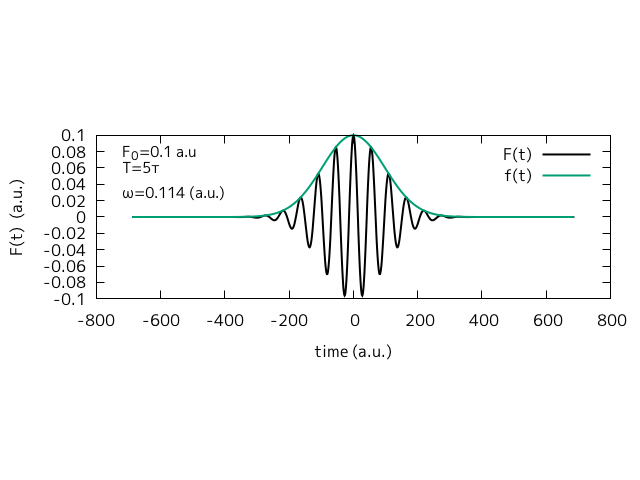
\includegraphics[scale=1., trim={0 20 0 120},clip]{images/field_01_114_5t.png}

%%\caption{Eigenvalues.}
%\label{fig:pemd_0114}
 \end{figure}


\end{minipage}
\end{textblock*}


\begin{textblock*}{700pt}(500pt,950pt)
\small

$I_0 = 3.51 \times 10^{16}\,{\rm W/cm^2} 
\longleftrightarrow F_0 = 1\,{\rm a.u.}$ 

\end{textblock*}




\begin{textblock*}{500pt}(1100pt,850pt)
 \mbox{\normalsize \textbf{Quantum Field}} \hspace{60pt}
 \begin{align}
&   \boldsymbol{\rm A}
  = \sum_\nu \boldsymbol{\rm A}_\nu \left( \hat{a}^{\dagger}_\nu 
    + \hat{a}_\nu\right), \nonumber \\
& \boldsymbol{F}(t) = -\frac{\partial \boldsymbol{A}(t)}{\partial t} \nonumber \\
& \mbox{If}\hspace{20pt} F_0 \gg 0.005\,{\rm a.u.}
 \longrightarrow \hspace{20pt}\mbox{\textbf{Classical treatment allowed}} \nonumber\\
& \hspace{20pt} \boldsymbol{F}(t) = \boldsymbol{F_0}\,e^{-(2t^\prime/\tau)^2} \cos (\omega t^\prime) \nonumber,\hspace{20pt}
\hspace{40pt}\mbox{\footnotesize $t^{\prime} = t - T/2, \hspace{20pt} 0 \leqslant t \leqslant T, 
\hspace{20pt}\tau = 2\pi n_{\rm oc}/\omega \hspace{20pt}, n_{\rm oc} =5, \hspace{20pt} T = n\tau$ \nonumber}
 \end{align}

\end{textblock*}



%\begin{textblock*}{500pt}(1700pt,850pt)
%%\centering
%%\rotatebox{90}{
% \begin{minipage}{0.6\linewidth}
% \begin{figure}[tp]
% 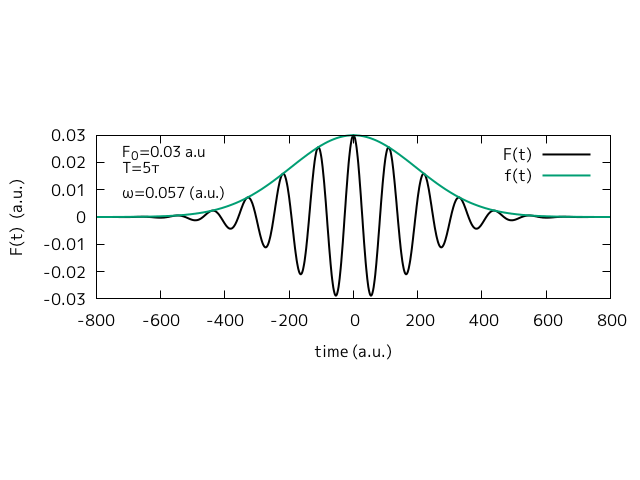
\includegraphics[scale=.8, trim={0 0 0 120},clip]{images/field_003_057_5t.png}
%
%%%\caption{Eigenvalues.}
%%\label{fig:pemd_0114}
% \end{figure}
%
%\end{minipage}
%\end{textblock*}




\begin{textblock*}{\textwidth}(1100pt,1250pt)
{\huge\textbf {4. Results}} \\\vspace{20pt}
{\normalsize{\textbf{Dipole moment of the particle \hspace{50pt}$\xrightarrow{\hspace{100pt}} $}}} 
\end{textblock*}


\begin{textblock*}{700pt}(1800pt,1200pt)
%\centering
%\rotatebox{90}{
%  \small \textbf{Basic strong field phenomena}
 \begin{minipage}{0.6\linewidth}
 \begin{figure}[tp]
 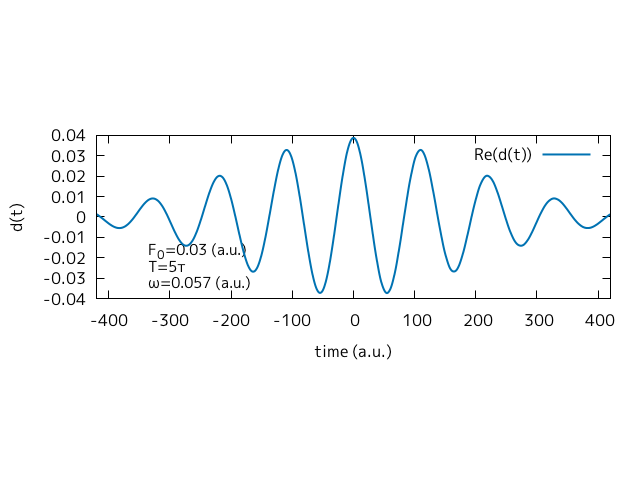
\includegraphics[scale=.8, trim={0 0 20 100},clip]{images/057_f003_d_t.png}

%%\caption{Eigenvalues.}
%\label{fig:pemd_0114}
 \end{figure}

\end{minipage}
\end{textblock*}


\begin{textblock*}{700pt}(1800pt,1360pt)
%\centering
%\rotatebox{90}{
%  \small \textbf{Basic strong field phenomena}
 \begin{minipage}{0.6\linewidth}
 \begin{figure}[tp]
 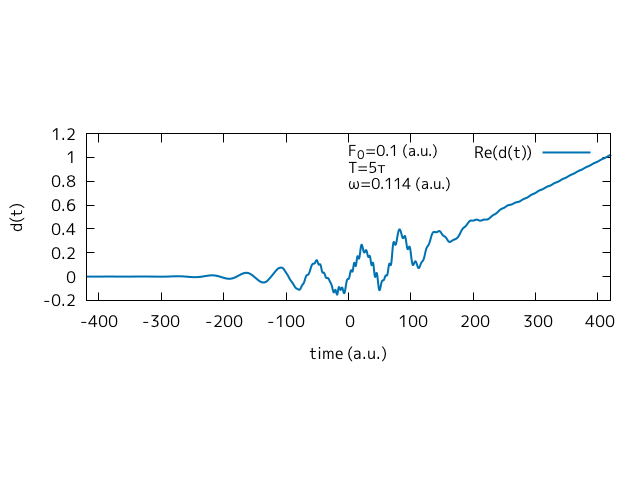
\includegraphics[scale=.8, trim={0 0 20 100},clip]{images/114_f01_d_t.png}

%%\caption{Eigenvalues.}
%\label{fig:pemd_0114}
 \end{figure}

\end{minipage}
\end{textblock*}


\begin{textblock*}{0.3\textwidth}(1100pt,1420pt)
{\normalsize{\textbf{Photoelectron momentum distribution 
and High harmonic generation}\hspace{50pt}$\downarrow$}} 
\end{textblock*}

\begin{textblock*}{700pt}(1050pt,1520pt)
%\centering
%\rotatebox{90}{
%  \small \textbf{Basic strong field phenomena}
 \begin{minipage}{0.6\linewidth}
 \begin{figure}[tp]
 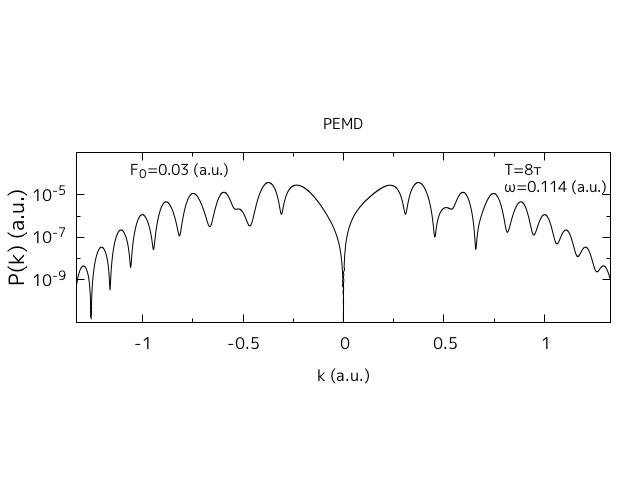
\includegraphics[scale=1., trim={0 0 20 150},clip]{images/114_f003_pemd.png}

%%\caption{Eigenvalues.}
%\label{fig:pemd_0114}
 \end{figure}

\end{minipage}
\end{textblock*}


\begin{textblock*}{700pt}(1050pt,1730pt)
%\centering
%\rotatebox{90}{
%  \small \textbf{Basic strong field phenomena}
 \begin{minipage}{0.6\linewidth}
 \begin{figure}[tp]
 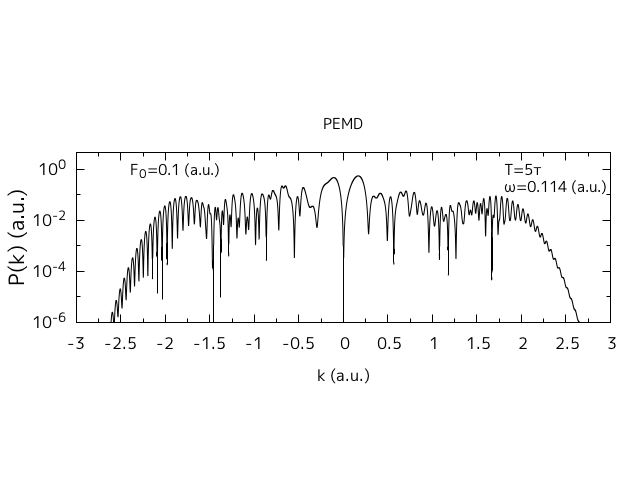
\includegraphics[scale=1., trim={0 0 20 150},clip]{images/114_f01_pemd.png}

%%\caption{Eigenvalues.}
%\label{fig:pemd_0114}
 \end{figure}

\end{minipage}
\end{textblock*}


\begin{textblock*}{700pt}(1050pt,1940pt)
%\centering
%\rotatebox{90}{
%  \small \textbf{Basic strong field phenomena}
 \begin{minipage}{0.6\linewidth}
 \begin{figure}[tp]
 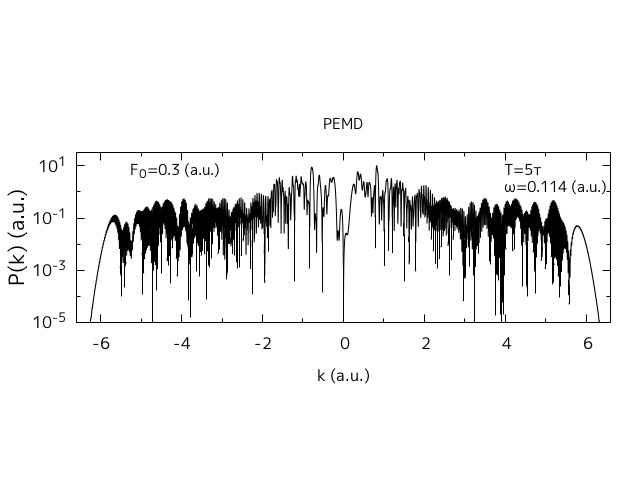
\includegraphics[scale=1., trim={0 0 20 150},clip]{images/114_f03_pemd.png}

%%\caption{Eigenvalues.}
%\label{fig:pemd_0114}
 \end{figure}

\end{minipage}
\end{textblock*}



\begin{textblock*}{700pt}(1050pt,2280pt)
%\centering
%\rotatebox{90}{
%  \small \textbf{Basic strong field phenomena}
 \begin{minipage}{0.6\linewidth}
 \begin{figure}[tp]
 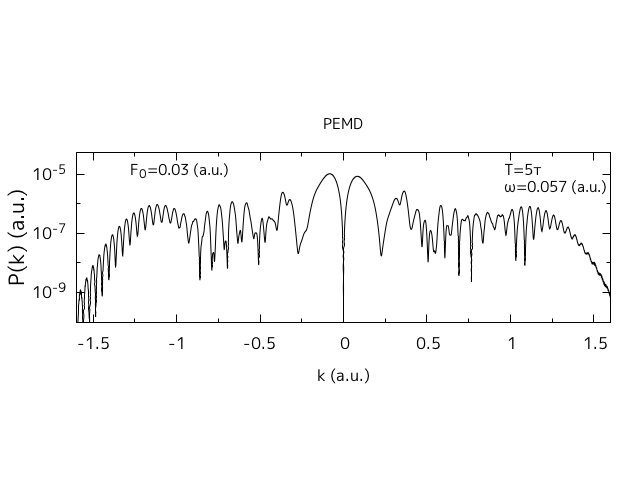
\includegraphics[scale=1., trim={0 0 20 150},clip]{images/057_f003_pemd.png}

%%\caption{Eigenvalues.}
%\label{fig:pemd_0114}
 \end{figure}

\end{minipage}
\end{textblock*}


\begin{textblock*}{700pt}(1050pt,2490pt)
%\centering
%\rotatebox{90}{
%  \small \textbf{Basic strong field phenomena}
 \begin{minipage}{0.6\linewidth}
 \begin{figure}[tp]
 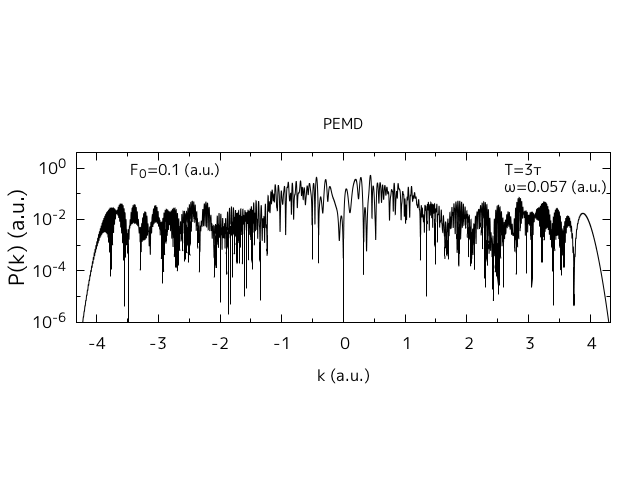
\includegraphics[scale=1., trim={0 0 20 150},clip]{images/057_f01_pemd.png}

%%\caption{Eigenvalues.}
%\label{fig:pemd_0114}
 \end{figure}

\end{minipage}
\end{textblock*}












\begin{textblock*}{700pt}(1700pt,1650pt)
%\centering
%\rotatebox{90}{
%  \small \textbf{Basic strong field phenomena}
 \begin{minipage}{0.6\linewidth}
 \begin{figure}[tp]
 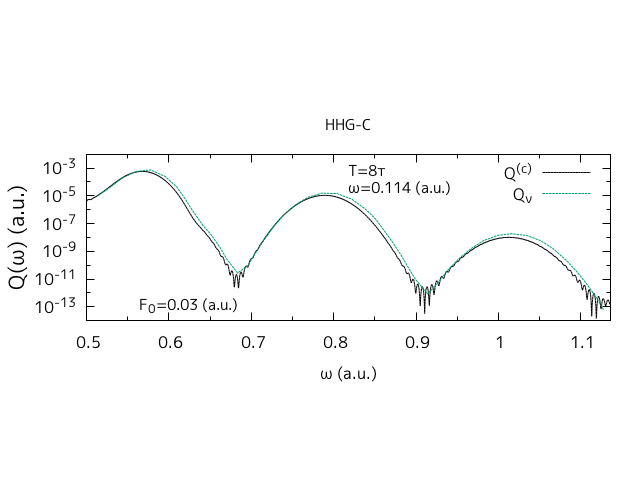
\includegraphics[scale=1., trim={0 0 0 150},clip]{images/114_f003_hhg.png}

%%\caption{Eigenvalues.}
%\label{fig:pemd_0114}
 \end{figure}


\end{minipage}
\end{textblock*}


\begin{textblock*}{700pt}(1700pt,1860pt)
%\centering
%\rotatebox{90}{
%  \small \textbf{Basic strong field phenomena}
 \begin{minipage}{0.6\linewidth}
 \begin{figure}[tp]
 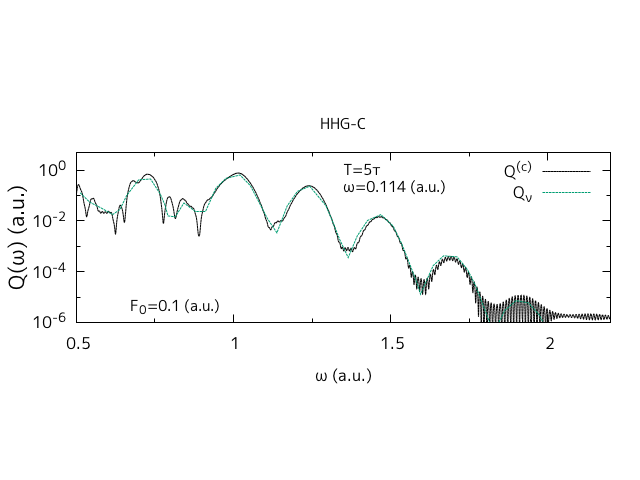
\includegraphics[scale=1., trim={0 0 0 150},clip]{images/114_f01_hhg.png}

%%\caption{Eigenvalues.}
%\label{fig:pemd_0114}
 \end{figure}


\end{minipage}
\end{textblock*}


\begin{textblock*}{700pt}(1700pt,2070pt)
%\centering
%\rotatebox{90}{
%  \small \textbf{Basic strong field phenomena}
 \begin{minipage}{0.6\linewidth}
 \begin{figure}[tp]
 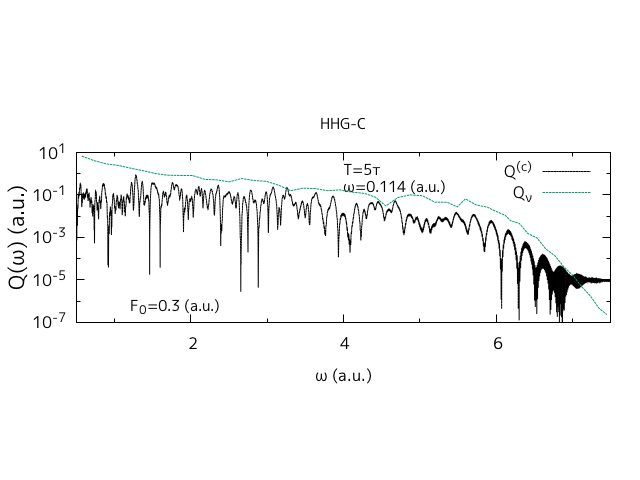
\includegraphics[scale=1., trim={0 0 0 144},clip]{images/114_f03_hhg.png}

%%\caption{Eigenvalues.}
%\label{fig:pemd_0114}
 \end{figure}


\end{minipage}
\end{textblock*}


\begin{textblock*}{700pt}(1700pt,2380pt)
%\centering
%\rotatebox{90}{
%  \small \textbf{Basic strong field phenomena}
 \begin{minipage}{0.6\linewidth}
 \begin{figure}[tp]
 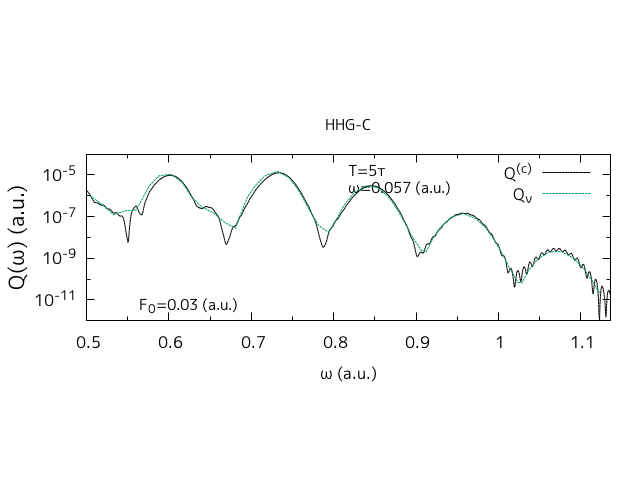
\includegraphics[scale=1., trim={0 0 0 150},clip]{images/057_f003_hhg.png}

%%\caption{Eigenvalues.}
%\label{fig:pemd_0114}
 \end{figure}


\end{minipage}
\end{textblock*}


\begin{textblock*}{700pt}(1700pt,2590pt)
%\centering
%\rotatebox{90}{
%  \small \textbf{Basic strong field phenomena}
 \begin{minipage}{0.6\linewidth}
 \begin{figure}[tp]
 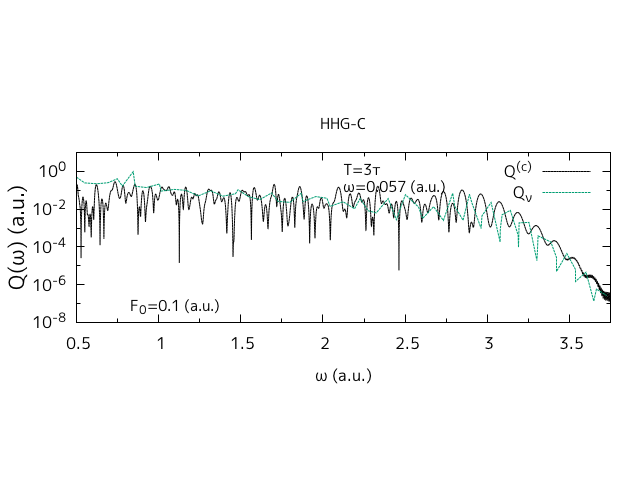
\includegraphics[scale=1., trim={0 0 0 150},clip]{images/057_f01_hhg.png}

%%\caption{Eigenvalues.}
%\label{fig:pemd_0114}
 \end{figure}


\end{minipage}
\end{textblock*}


\begin{textblock*}{600pt}(1750pt,2325pt)
\scriptsize
\centering 
\textbf{
Quantum correction required for 
$\boldsymbol{F_0 \geqslant 0.3\,{\rm a.u.}}$}
\end{textblock*}




\begin{textblock*}{0.5\textwidth}(1100pt,2850pt)
{\huge\textbf {5. Conclusion}} \\\vspace{30pt}
\begin{itemize}
\small
\item The classical ansatz used to evaluate HHG spectra 
ceases to be a good approximation for field strengths approaching unity
\item Since lasers of intensity greater than 
$I_0$ are now available, 
a more appropriate theoretical treatment for HHG is highly desirable
\vspace{20pt}
\item The present study aims at extending this previous result 
to realistic  atomic system 
\end{itemize}
\end{textblock*}


\end{frame}
\end{document}
